\section{editrecord Class Reference}
\label{classeditrecord}\index{editrecord@{editrecord}}
{\tt \#include $<$editrecord.h$>$}

Collaboration diagram for editrecord:\begin{figure}[H]
\begin{center}
\leavevmode
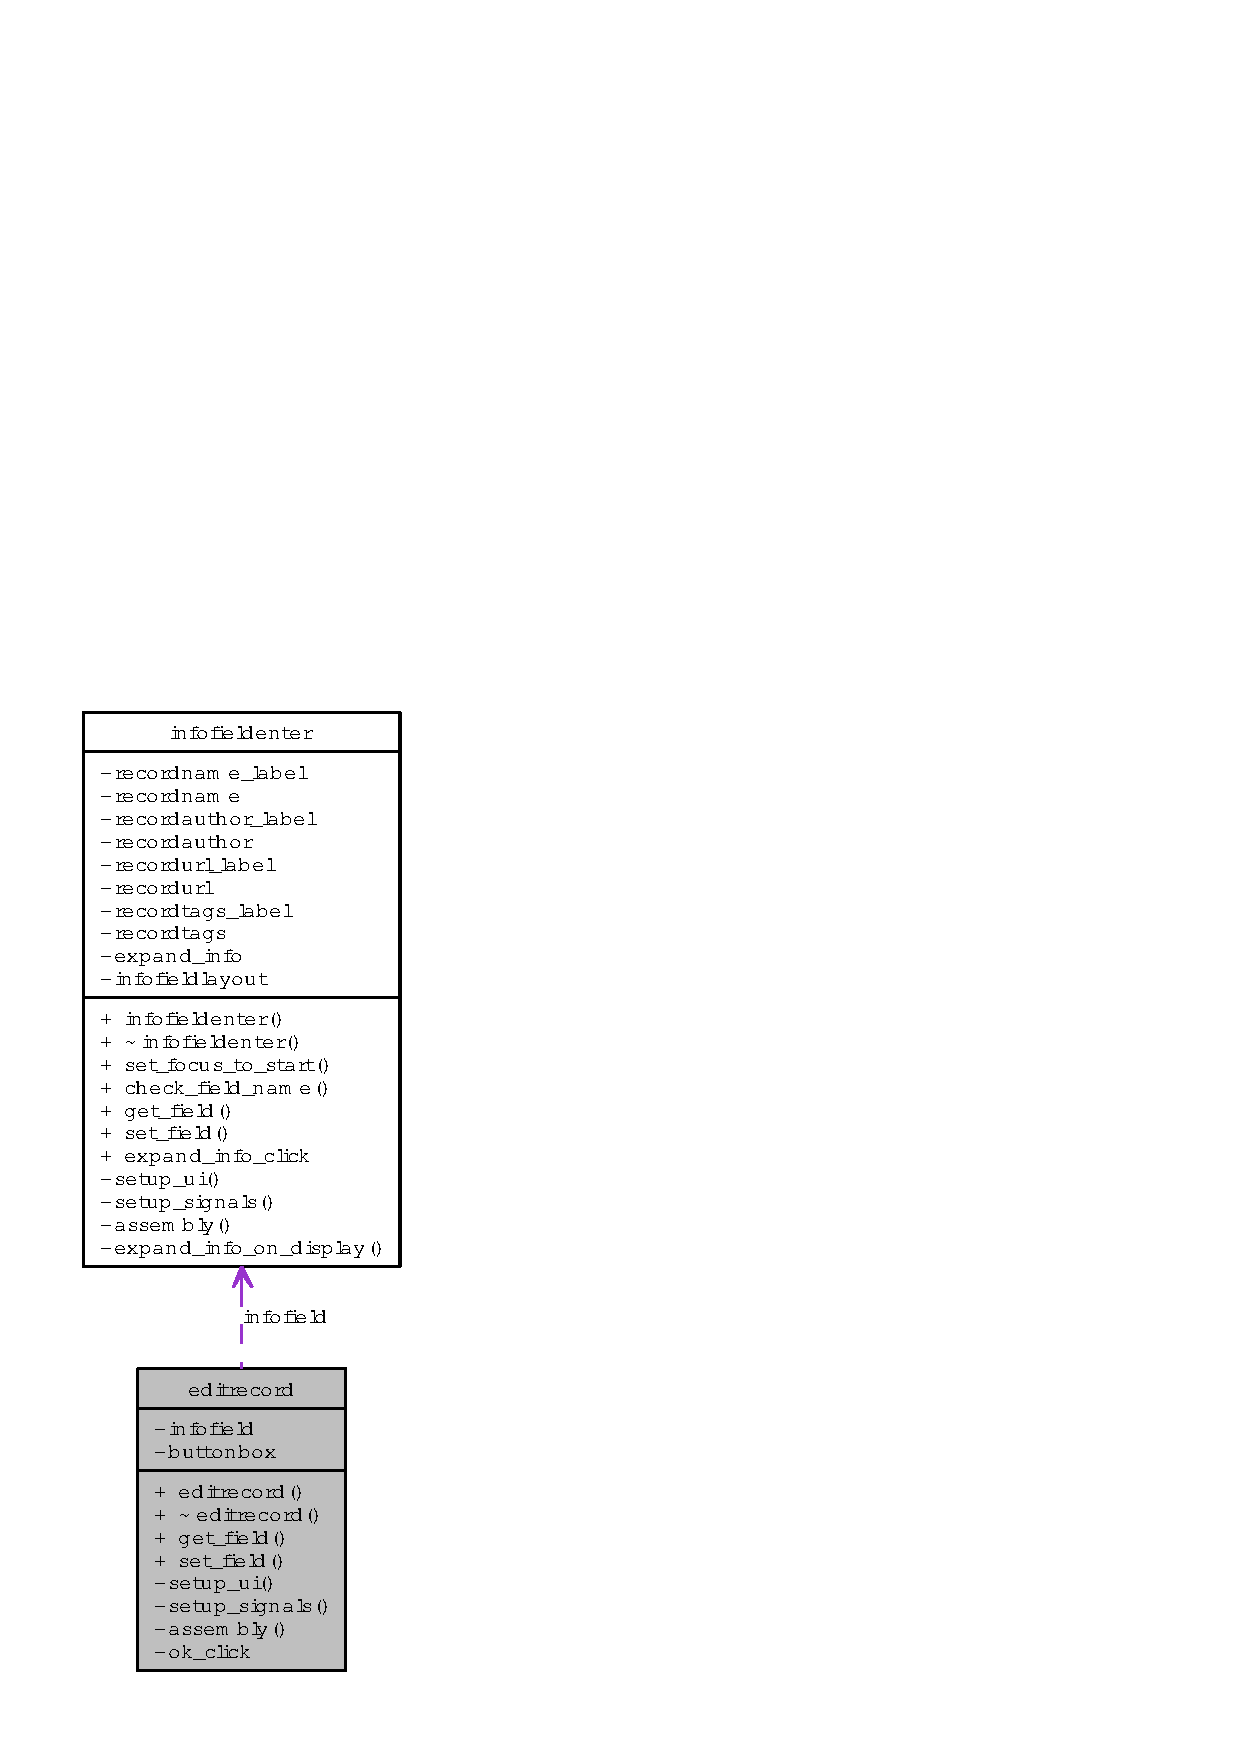
\includegraphics[width=98pt]{classeditrecord__coll__graph}
\end{center}
\end{figure}
\subsection*{Public Member Functions}
\begin{CompactItemize}
\item 
{\bf editrecord} (QWidget $\ast$parent=0, Qt::WFlags f=0)
\item 
{\bf $\sim$editrecord} ()
\item 
QString {\bf get\_\-field} (QString name)
\item 
void {\bf set\_\-field} (QString name, QString value)
\end{CompactItemize}
\subsection*{Private Slots}
\begin{CompactItemize}
\item 
void {\bf ok\_\-click} (void)
\end{CompactItemize}
\subsection*{Private Member Functions}
\begin{CompactItemize}
\item 
void {\bf setup\_\-ui} (void)
\item 
void {\bf setup\_\-signals} (void)
\item 
void {\bf assembly} (void)
\end{CompactItemize}
\subsection*{Private Attributes}
\begin{CompactItemize}
\item 
{\bf infofieldenter} $\ast$ {\bf infofield}
\item 
QDialog\-Button\-Box $\ast$ {\bf buttonbox}
\end{CompactItemize}


\subsection{Detailed Description}




Definition at line 15 of file editrecord.h.

\subsection{Constructor \& Destructor Documentation}
\index{editrecord@{editrecord}!editrecord@{editrecord}}
\index{editrecord@{editrecord}!editrecord@{editrecord}}
\subsubsection{\setlength{\rightskip}{0pt plus 5cm}editrecord::editrecord (QWidget $\ast$ {\em parent} = {\tt 0}, Qt::WFlags {\em f} = {\tt 0})}\label{classeditrecord_854413f1af75438302e9e242b3c4a130}




Definition at line 12 of file editrecord.cpp.

References assembly(), setup\_\-signals(), and setup\_\-ui().

Here is the call graph for this function:\begin{figure}[H]
\begin{center}
\leavevmode
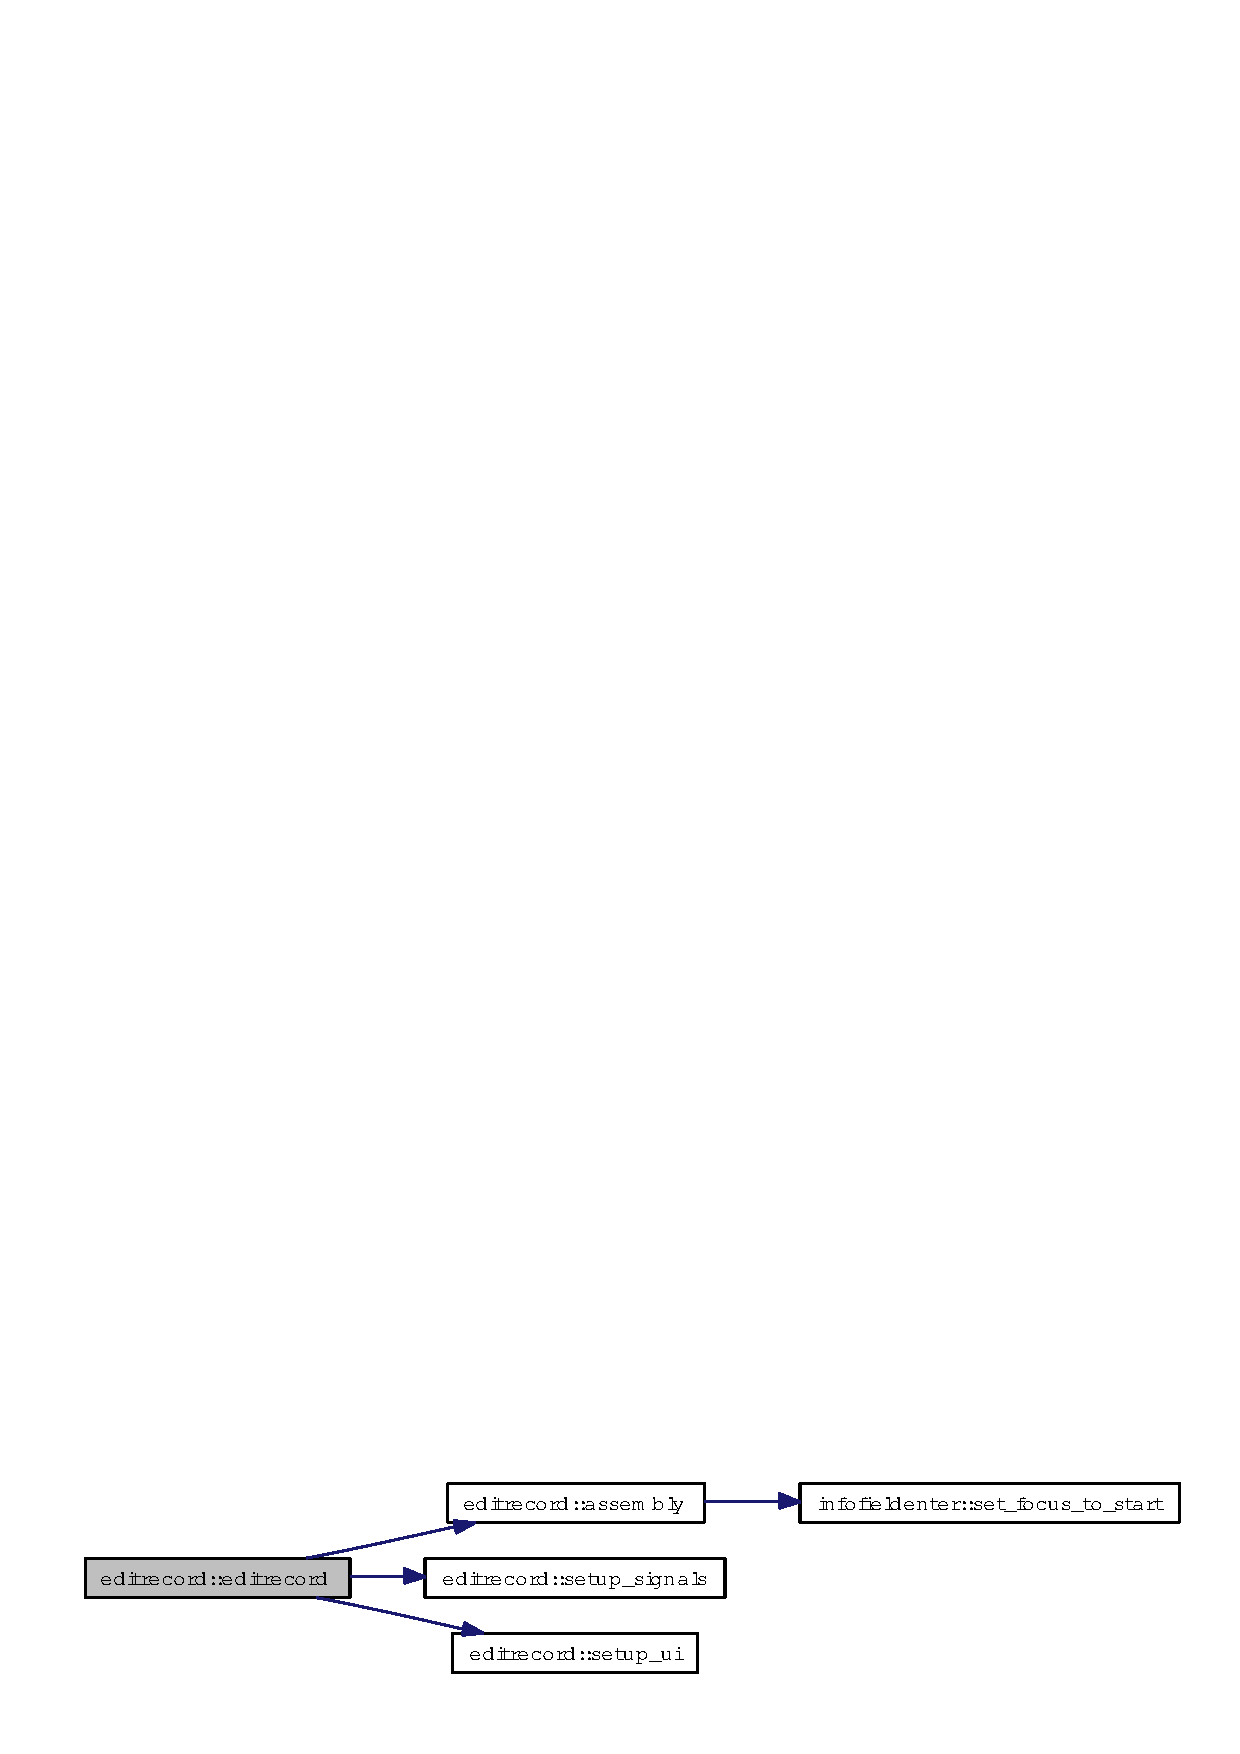
\includegraphics[width=285pt]{classeditrecord_854413f1af75438302e9e242b3c4a130_cgraph}
\end{center}
\end{figure}
\index{editrecord@{editrecord}!~editrecord@{$\sim$editrecord}}
\index{~editrecord@{$\sim$editrecord}!editrecord@{editrecord}}
\subsubsection{\setlength{\rightskip}{0pt plus 5cm}editrecord::$\sim$editrecord ()}\label{classeditrecord_4dfd76bc8e329941b5cb0df2bfce5438}




Definition at line 19 of file editrecord.cpp.

\subsection{Member Function Documentation}
\index{editrecord@{editrecord}!get_field@{get\_\-field}}
\index{get_field@{get\_\-field}!editrecord@{editrecord}}
\subsubsection{\setlength{\rightskip}{0pt plus 5cm}QString editrecord::get\_\-field (QString {\em name})}\label{classeditrecord_07fa56843727ad158ae073c9b40909e6}




Definition at line 91 of file editrecord.cpp.

References infofieldenter::check\_\-field\_\-name(), critical\_\-error(), infofieldenter::get\_\-field(), and infofield.

Referenced by recordtablescreen::edit\_\-field\_\-context().

Here is the call graph for this function:\begin{figure}[H]
\begin{center}
\leavevmode
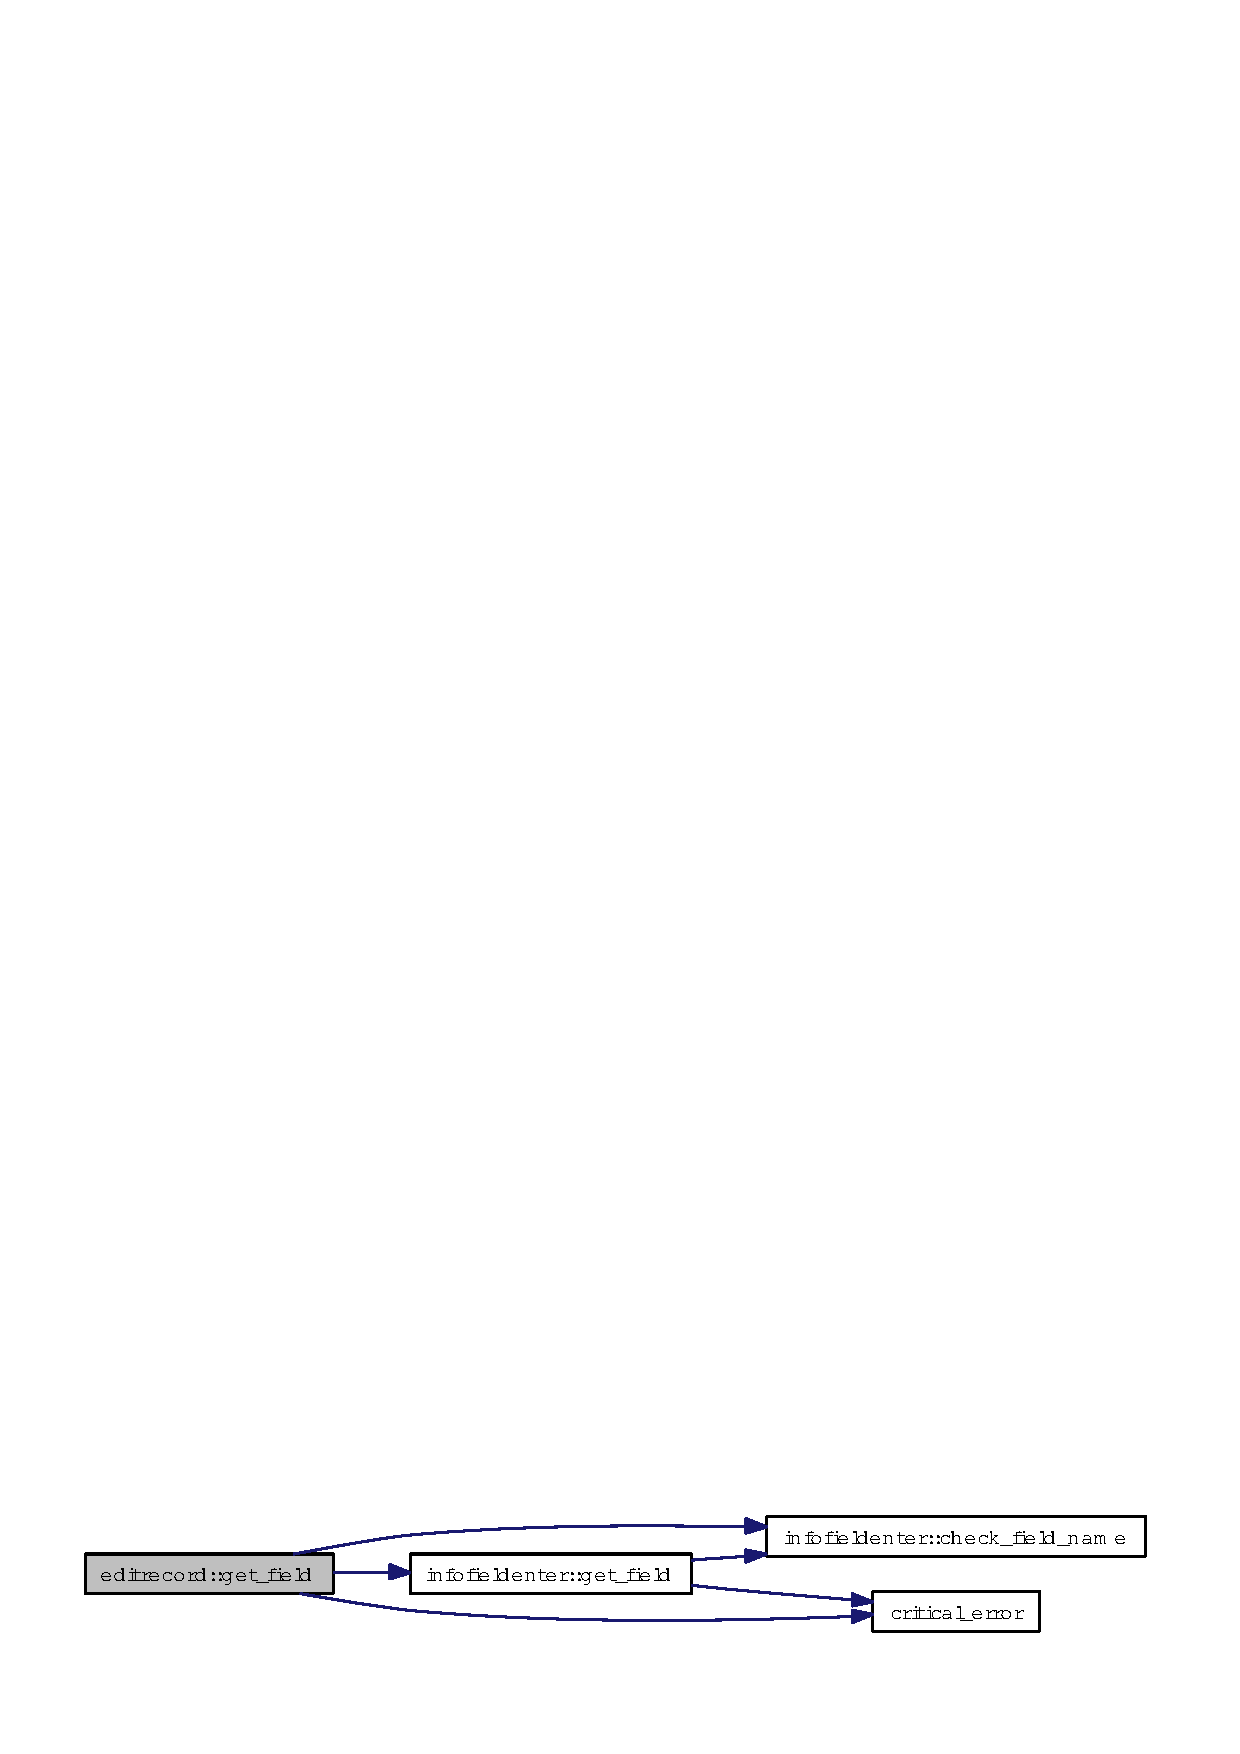
\includegraphics[width=277pt]{classeditrecord_07fa56843727ad158ae073c9b40909e6_cgraph}
\end{center}
\end{figure}
\index{editrecord@{editrecord}!set_field@{set\_\-field}}
\index{set_field@{set\_\-field}!editrecord@{editrecord}}
\subsubsection{\setlength{\rightskip}{0pt plus 5cm}void editrecord::set\_\-field (QString {\em name}, QString {\em value})}\label{classeditrecord_7e6e9990768cb64f0e73e3f7b94fa5a1}




Definition at line 102 of file editrecord.cpp.

References infofieldenter::check\_\-field\_\-name(), critical\_\-error(), infofield, and infofieldenter::set\_\-field().

Referenced by recordtablescreen::edit\_\-field\_\-context().

Here is the call graph for this function:\begin{figure}[H]
\begin{center}
\leavevmode
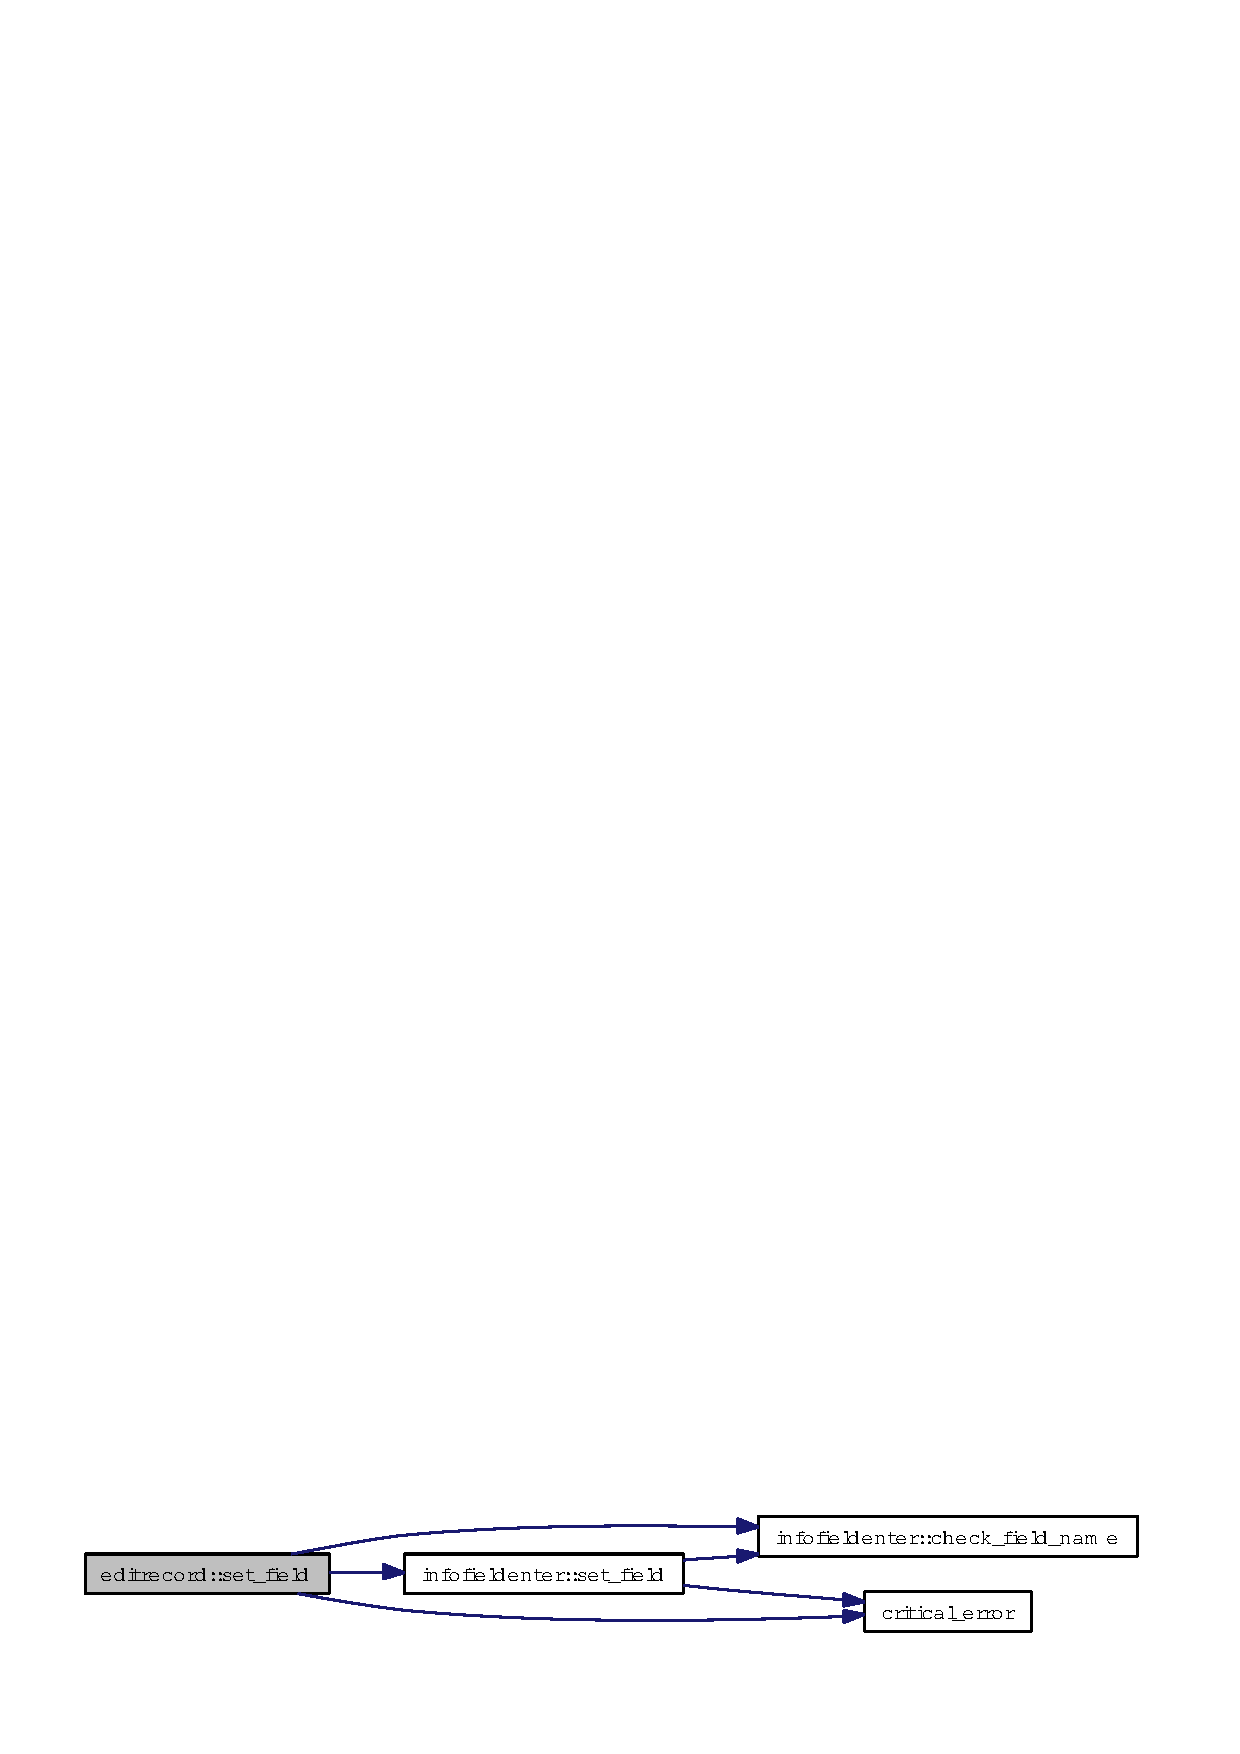
\includegraphics[width=275pt]{classeditrecord_7e6e9990768cb64f0e73e3f7b94fa5a1_cgraph}
\end{center}
\end{figure}
\index{editrecord@{editrecord}!ok_click@{ok\_\-click}}
\index{ok_click@{ok\_\-click}!editrecord@{editrecord}}
\subsubsection{\setlength{\rightskip}{0pt plus 5cm}void editrecord::ok\_\-click (void)\hspace{0.3cm}{\tt  [private, slot]}}\label{classeditrecord_be9bea72d91d0a91f6b4c09402329f76}




Definition at line 69 of file editrecord.cpp.

References infofieldenter::get\_\-field(), and infofield.

Referenced by setup\_\-signals().\index{editrecord@{editrecord}!setup_ui@{setup\_\-ui}}
\index{setup_ui@{setup\_\-ui}!editrecord@{editrecord}}
\subsubsection{\setlength{\rightskip}{0pt plus 5cm}void editrecord::setup\_\-ui (void)\hspace{0.3cm}{\tt  [private]}}\label{classeditrecord_4b8901e5eb8582c21726876dc0bb435b}




Definition at line 25 of file editrecord.cpp.

References buttonbox, and infofield.

Referenced by editrecord().

Here is the caller graph for this function:\begin{figure}[H]
\begin{center}
\leavevmode
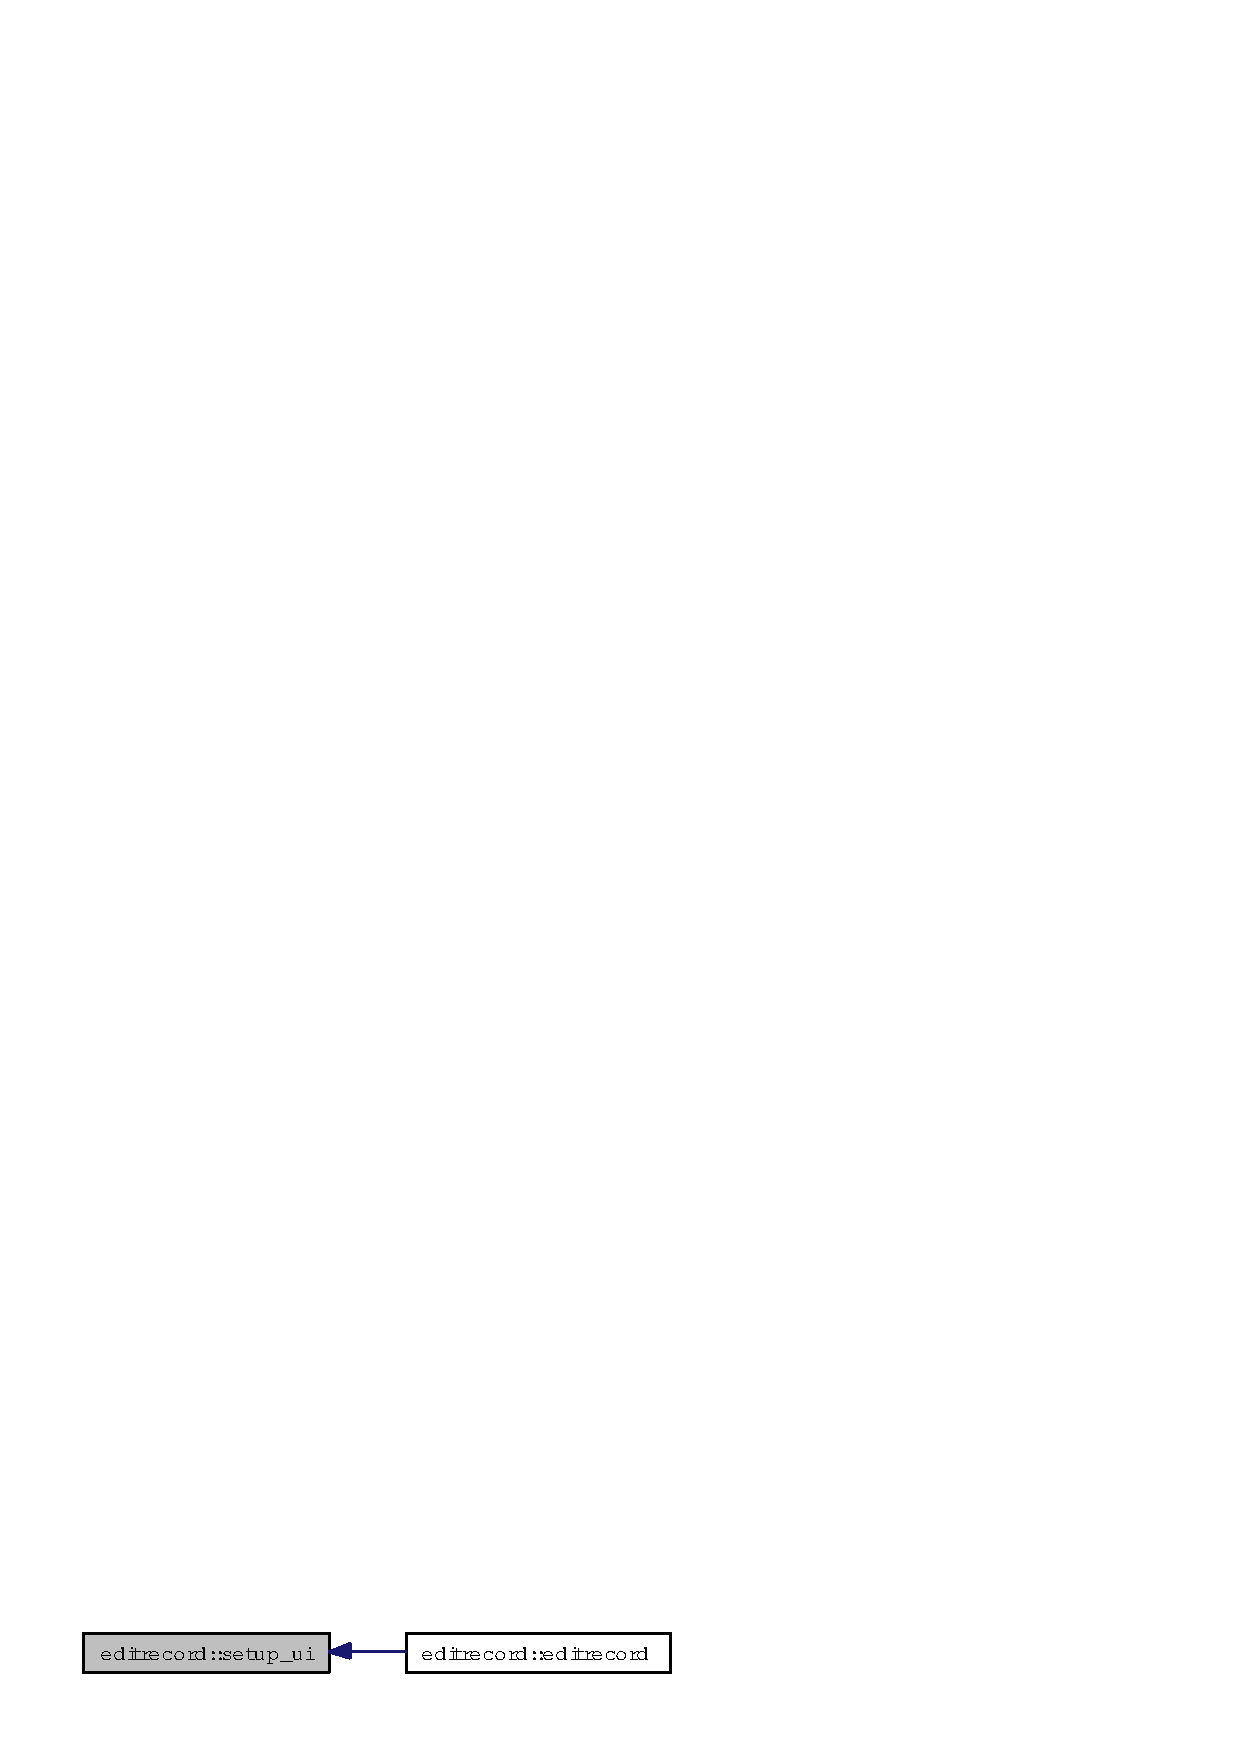
\includegraphics[width=163pt]{classeditrecord_4b8901e5eb8582c21726876dc0bb435b_icgraph}
\end{center}
\end{figure}
\index{editrecord@{editrecord}!setup_signals@{setup\_\-signals}}
\index{setup_signals@{setup\_\-signals}!editrecord@{editrecord}}
\subsubsection{\setlength{\rightskip}{0pt plus 5cm}void editrecord::setup\_\-signals (void)\hspace{0.3cm}{\tt  [private]}}\label{classeditrecord_753eba2e913f71ba5106b2463b6e468d}




Definition at line 36 of file editrecord.cpp.

References buttonbox, and ok\_\-click().

Referenced by editrecord().

Here is the caller graph for this function:\begin{figure}[H]
\begin{center}
\leavevmode
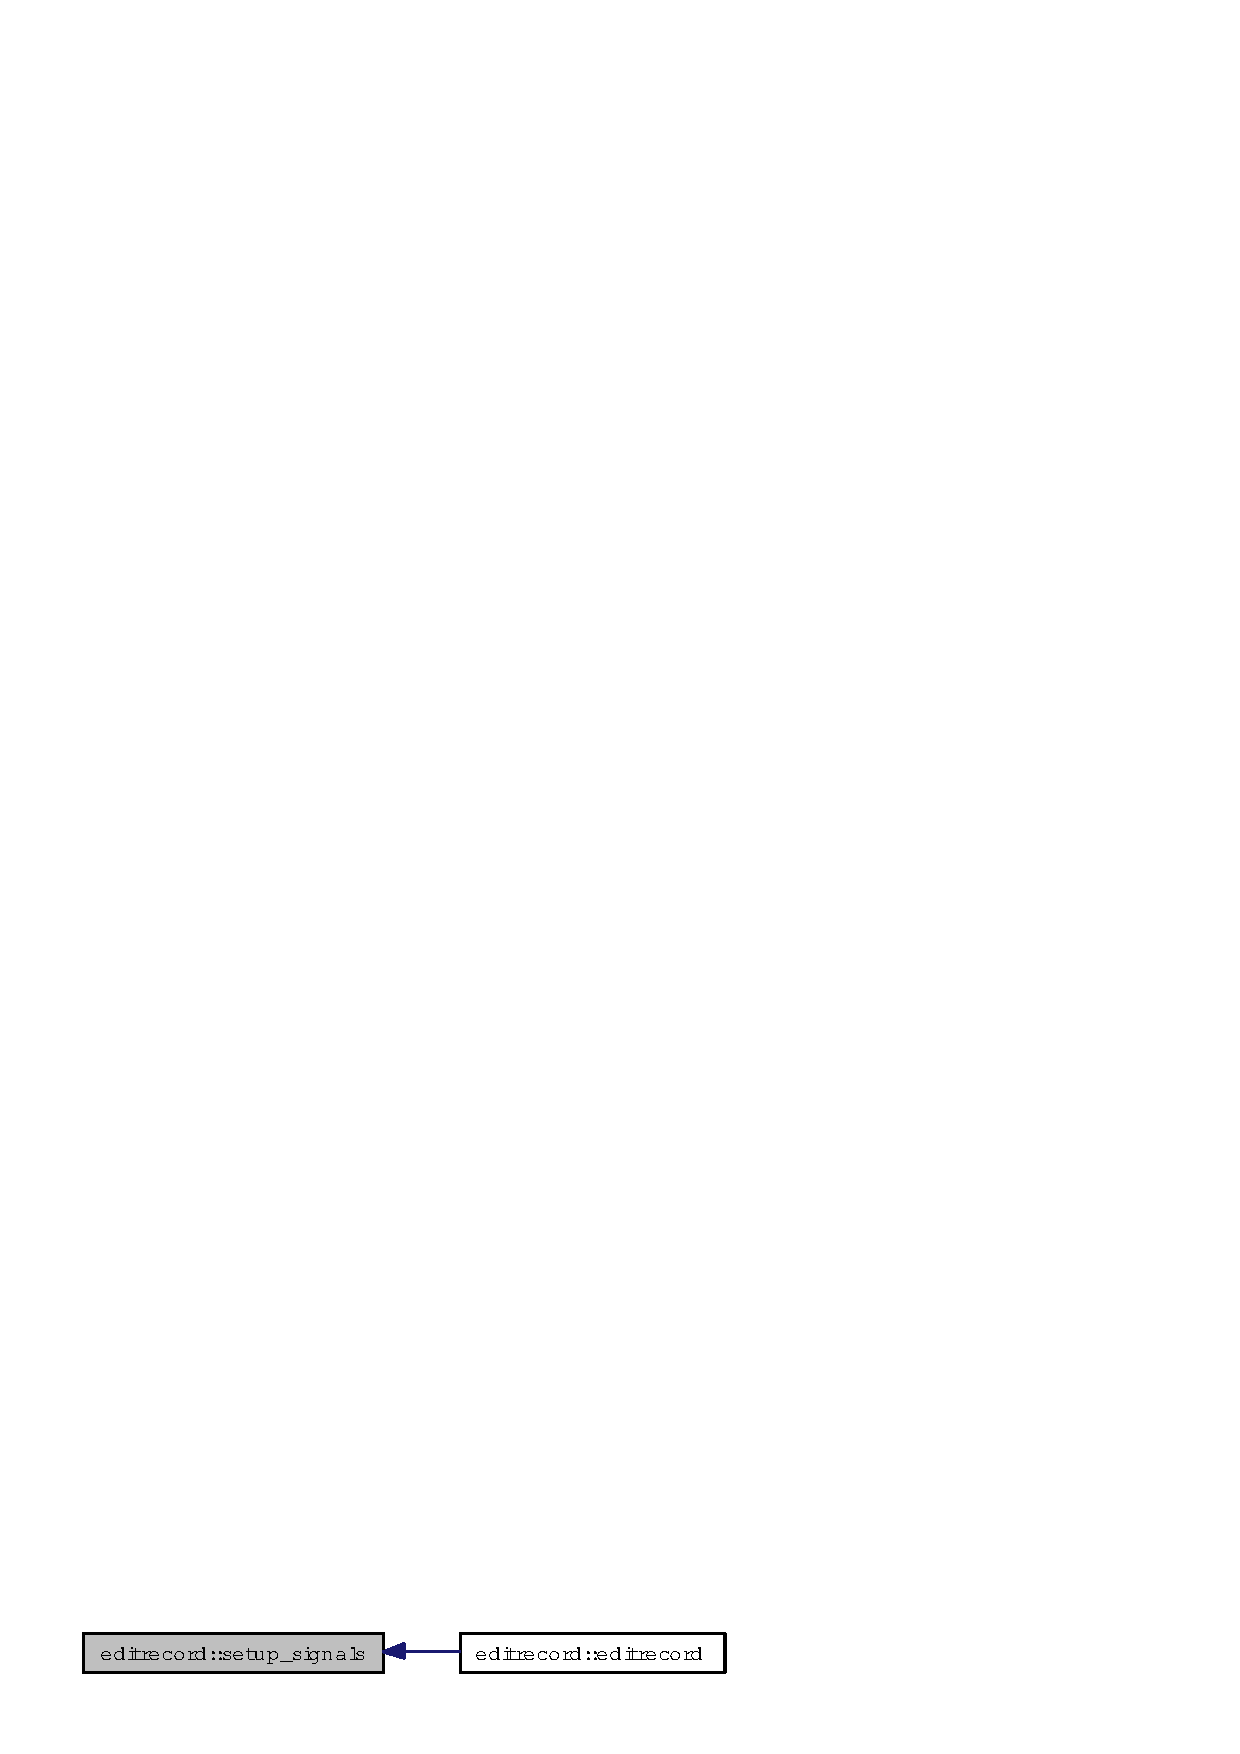
\includegraphics[width=176pt]{classeditrecord_753eba2e913f71ba5106b2463b6e468d_icgraph}
\end{center}
\end{figure}
\index{editrecord@{editrecord}!assembly@{assembly}}
\index{assembly@{assembly}!editrecord@{editrecord}}
\subsubsection{\setlength{\rightskip}{0pt plus 5cm}void editrecord::assembly (void)\hspace{0.3cm}{\tt  [private]}}\label{classeditrecord_21b3d76e14217b64e280c2b28a3f3175}




Definition at line 42 of file editrecord.cpp.

References buttonbox, infofield, and infofieldenter::set\_\-focus\_\-to\_\-start().

Referenced by editrecord().

Here is the call graph for this function:\begin{figure}[H]
\begin{center}
\leavevmode
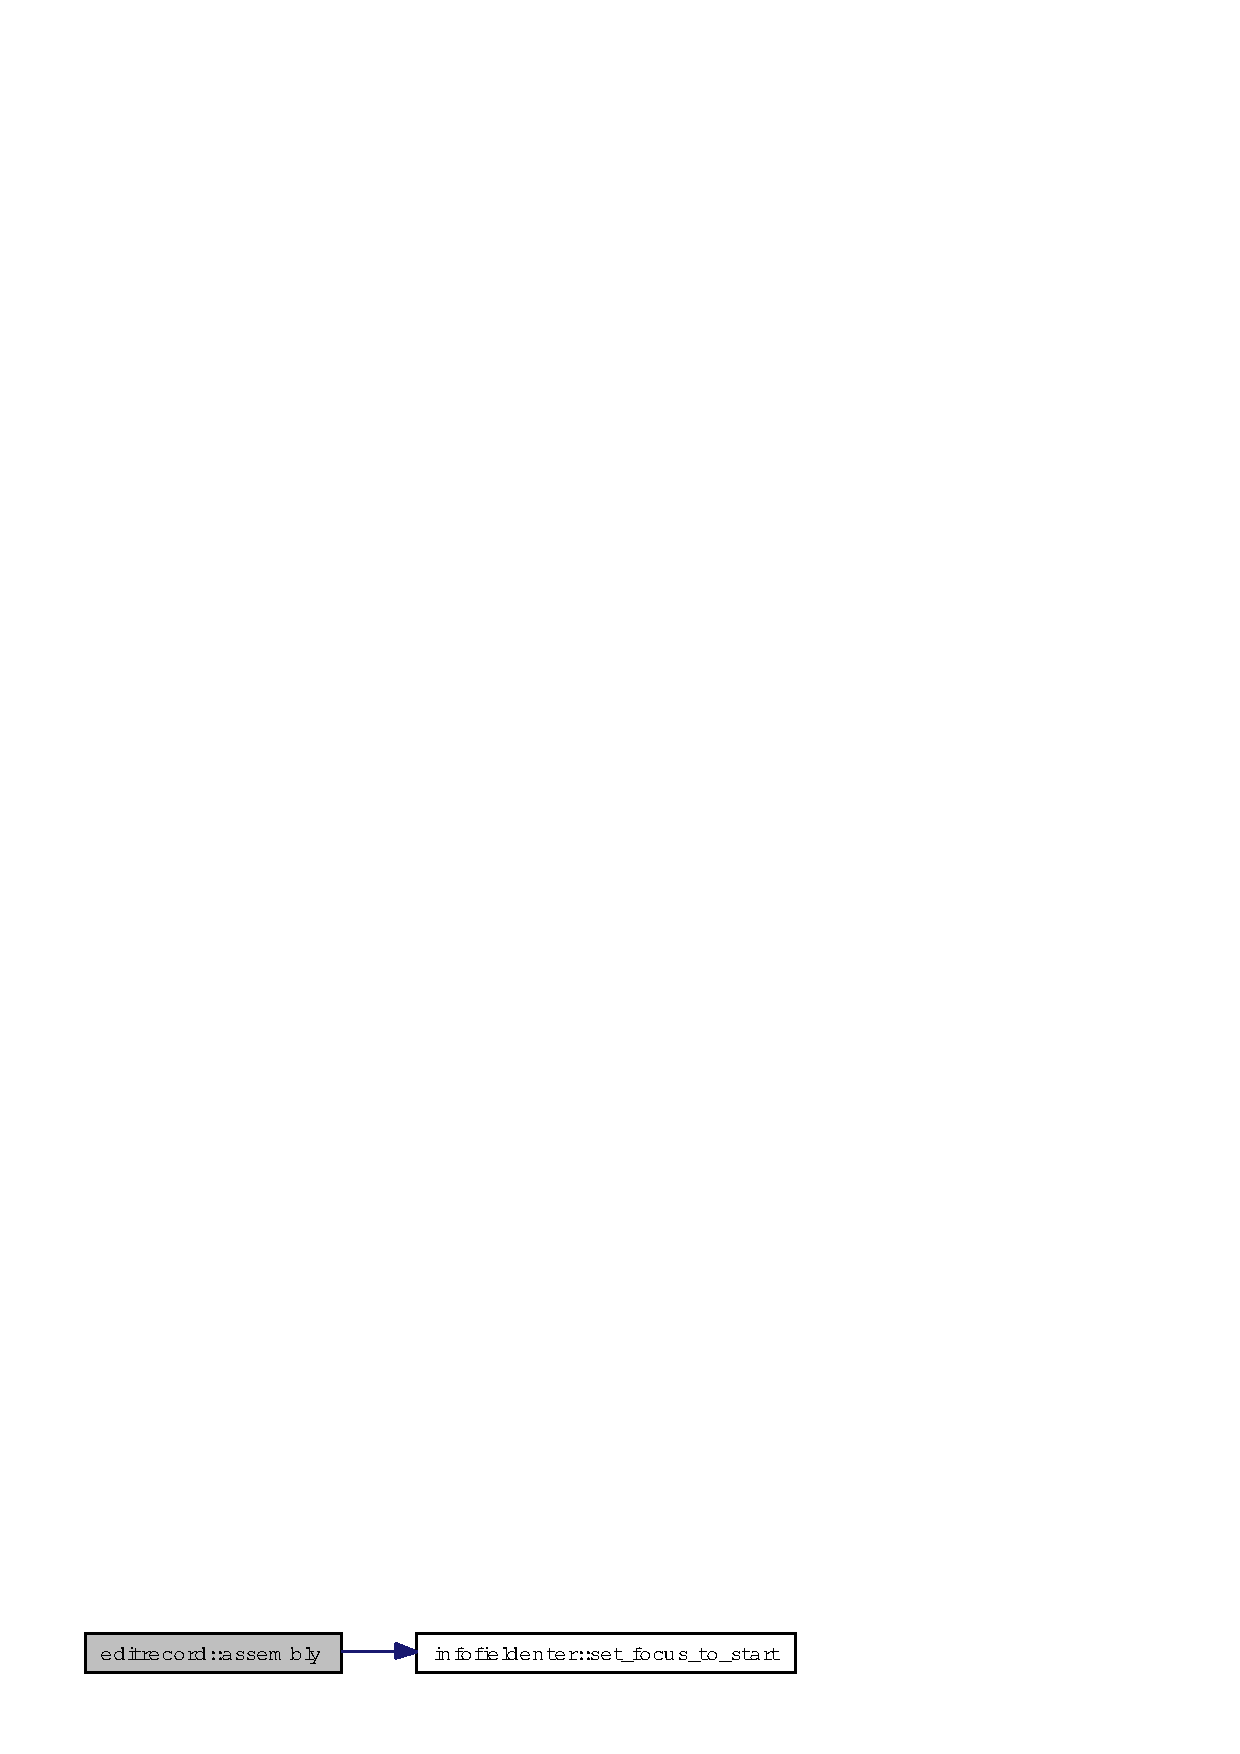
\includegraphics[width=193pt]{classeditrecord_21b3d76e14217b64e280c2b28a3f3175_cgraph}
\end{center}
\end{figure}


Here is the caller graph for this function:\begin{figure}[H]
\begin{center}
\leavevmode
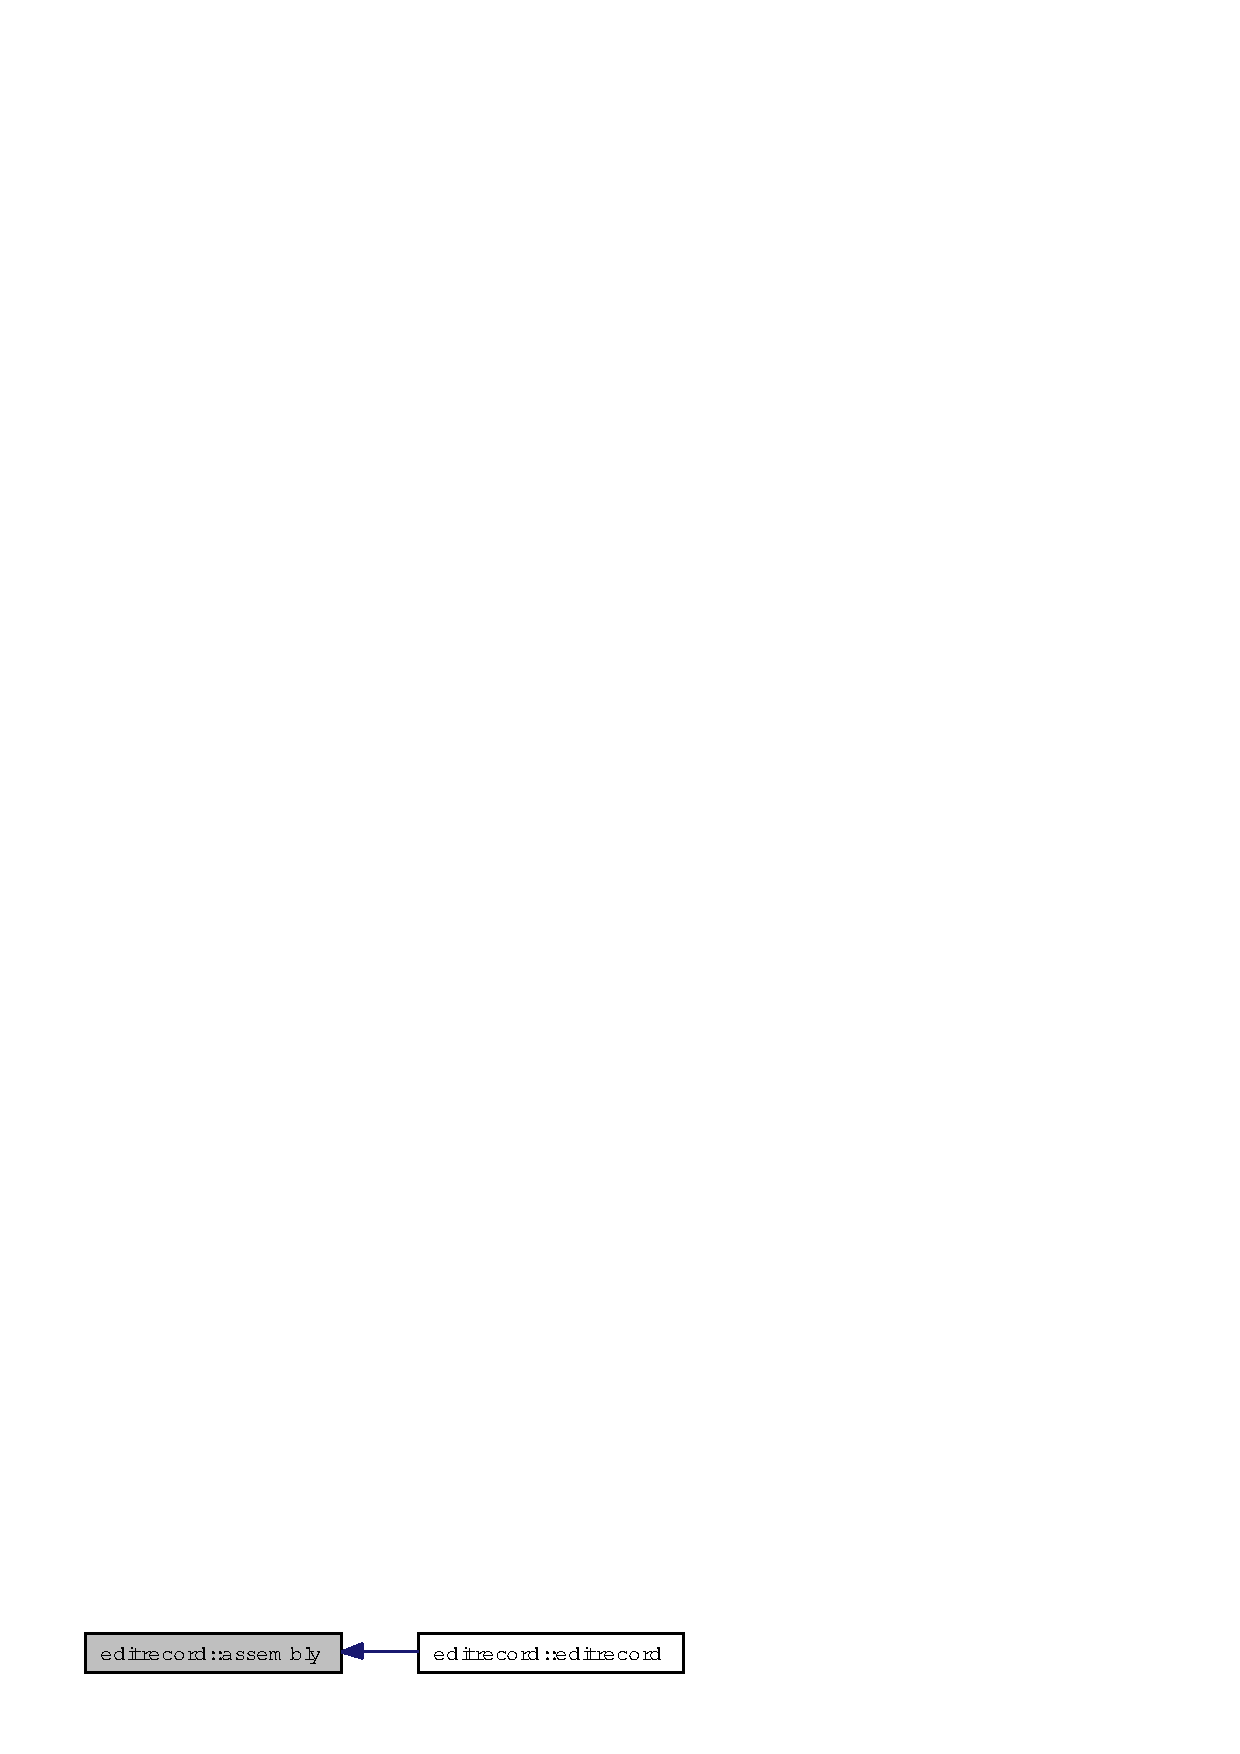
\includegraphics[width=166pt]{classeditrecord_21b3d76e14217b64e280c2b28a3f3175_icgraph}
\end{center}
\end{figure}


\subsection{Member Data Documentation}
\index{editrecord@{editrecord}!infofield@{infofield}}
\index{infofield@{infofield}!editrecord@{editrecord}}
\subsubsection{\setlength{\rightskip}{0pt plus 5cm}{\bf infofieldenter}$\ast$ {\bf editrecord::infofield}\hspace{0.3cm}{\tt  [private]}}\label{classeditrecord_0f1df1474362ce3fb91219279aad9c3c}




Definition at line 33 of file editrecord.h.

Referenced by assembly(), get\_\-field(), ok\_\-click(), set\_\-field(), and setup\_\-ui().\index{editrecord@{editrecord}!buttonbox@{buttonbox}}
\index{buttonbox@{buttonbox}!editrecord@{editrecord}}
\subsubsection{\setlength{\rightskip}{0pt plus 5cm}QDialog\-Button\-Box$\ast$ {\bf editrecord::buttonbox}\hspace{0.3cm}{\tt  [private]}}\label{classeditrecord_fd6ed719dfca0229e45aadbac28eff6b}




Definition at line 35 of file editrecord.h.

Referenced by assembly(), setup\_\-signals(), and setup\_\-ui().

The documentation for this class was generated from the following files:\begin{CompactItemize}
\item 
{\bf editrecord.h}\item 
{\bf editrecord.cpp}\end{CompactItemize}
